%% EDM2018 
%%%%%%%%%%%%%%%%%%%%%%%%%%%%%%%%%%%%%%%%%%%%%%%%%%%%%%%%%%%%%%%%%%%%%%%%%%%%%%%%%%%%%%%%%%%%%%%%%%%

%% document class
%\documentclass{beamer}
%\documentclass[aspectratio=169]{beamer}
\documentclass[handout]{beamer}

%% packages
\usepackage[utf8]{inputenc}
\usepackage{multicol}
\usepackage{amsmath}% http://ctan.org/pkg/amsmath
\usepackage{kbordermatrix}% http://www.hss.caltech.edu/~kcb/TeX/kbordermatrix.sty
\usepackage{slashbox}
\usepackage{multirow}
\usepackage{mathrsfs}
\usepackage{graphicx}
\usepackage{pdfpages}

%% page settings
%% Theme
\usetheme{Berkeley} % theme for slides
%\usetheme{Frankfurt}
%\usetheme{Madrid}

%% Colors
%\usecolortheme{rose} % color for slides
\usecolortheme{default}
%\definecolor{c1}{rgb}{0,0.7,0.6} % some green
%\definecolor{c2}{rgb}{0.9,0.9,0.9} % some gray
%% see http://www.sharelatex.com/learn/Beamer
%\setbeamercolor*{palette primary}{fg=white,bg=c1} % upper part
%\setbeamercolor*{palette secondary}{bg=c2} % left part (background)
%\setbeamercolor*{sidebar left}{fg=white,bg=c1} % left part with links
%\setbeamerfont{section number projected}{ % section numbers
%  family=\rmfamily,
%  series=\bfseries,
%  size=\normalsize
%  }
%\setbeamercolor{section number projected}{bg=c1} % color of section numbers and others (fg: Fontm, bg:Hintergrund)
%\setbeamercolor{item projected}{bg=c1}
%\setbeamercolor{itemize item}{fg=c1}
%\setbeamercolor{author in sidebar}{fg=white}
%\setbeamercolor{footlinecolor}{fg=black,bg=c2}

%% Fonts
\usefonttheme{professionalfonts} % changes fonts

%% Foot
\usenavigationsymbolstemplate{} % deafult controls off
\setbeamertemplate{footline}[frame number] % slide number at the bottom
%\setbeamertemplate{footline}
%{%
%	\leavevmode%
%	\hbox{%
%	\begin{beamercolorbox}[wd=.3\paperwidth,ht=5ex,dp=1.5ex,left,leftskip=2mm]{footlinecolor}%
%		Foot information on the left over several lines
%	\end{beamercolorbox}%
%	\begin{beamercolorbox}[wd=.5\paperwidth,ht=5ex,dp=1.5ex,left,leftskip=2mm]{footlinecolor}%
%		Next foot part
%	\end{beamercolorbox}%
%	\begin{beamercolorbox}[wd=.2\paperwidth,ht=5ex,dp=1.5ex,right,rightskip=2mm]{footlinecolor}%
%		\insertframenumber{} / \inserttotalframenumber%
%	\end{beamercolorbox}%
%	}%
%	\vskip0pt%
%}

%% new commands
\newcommand{\cm}[1]{{\tt \textcolor{orange}{#1}}}
\newcommand{\wl}[2]{\href{#2}{\textcolor{blue}{#1}}}
\newcommand{\att}[2]{\href{#2}{\textcolor{blue}{#1}}}
\newcommand\scalemath[2]{\scalebox{#1}{\mbox{\ensuremath{\displaystyle #2}}}}
\newcommand\norm[1]{\left\lVert#1\right\rVert}

%%%%%%%%%%%%%%%%%%%%%%%%%%%%%%%%%%%%%%%%%%%%%%%%%%%%%%%%%%%%%%%%%%%%%%%%%%%%%%%%%%%%%%%%%%%%%%%%%%%

\begin{document}

%%%%%%%%%%%%%%%%%%%%%%%%%%%%%%%%%%%%%%%%%%%%%%%%%%%%%%%%%%%%%%%%%%%%%%%%%%%%%%%%%%%%%%%%%%%%%%%%%%%
%%%%%%%%%%%%%%%%%%%%%%%%%%%%%%%%%%%%%%%%%%%%%%%%%%%%%%%%%%%%%%%%%%%%%%%%%%%%%%%%%%%%%%%%%%%%%%%%%%%
%%%%%%%%%%%%%%%%%%%%%%%%%%%%%%%%%%%%%%%%%%%%%%%%%%%%%%%%%%%%%%%%%%%%%%%%%%%%%%%%%%%%%%%%%%%%%%%%%%%

\author[Peng Xu \& Michel Demarais]{\textbf {Peng Xu, Michel Desmarais}}
\title[Title]{An Empirical Research on Identifiability and Q-matrix Design for DINA model}
\titlegraphic{
\includegraphics[width=0.35\textwidth]{figures/polytechnique}}
\institute{Département de Génie Informatique et Génie Logiciel}
\date{July 15, 2018}
\frame{\titlepage}


%%%%%%%%%%%%%%%%%%%%%%%%%%%%%%%%%%%%%%%%%%%%%%%%%%%%%%%%%%%%%%%%%%%%%%%%%%%%%%%%%%%%%%%%%%%%%%%%%%%

\begin{frame}{Table of contents}
\begin{multicols}{2}
  \tableofcontents
\end{multicols}
\end{frame}

%%%%%%%%%%%%%%%%%%%%%%%%%%%%%%%%%%%%%%%%%%%%%%%%%%%%%%%%%%%%%%%%%%%%%%%%%%%%%%%%%%%%%%%%%%%%%%%%%%%
%%%%%%%%%%%%%%%%%%%%%%%%%%%%%%%%%%%%%%%%%%%%%%%%%%%%%%%%%%%%%%%%%%%%%%%%%%%%%%%%%%%%%%%%%%%%%%%%%%%

\section{Introduction}
%\begin{frame}{Table of contents}
%\begin{multicols}{2}
%  \tableofcontents[currentsection,hidesubsections]
%\end{multicols}
%\end{frame}

%%%%%%%%%%%%%%%%%%%%%%%%%%%%%%%%%%%%%%%%%%%%%%%%%%%%%%%%%%%%%%%%%%%%%%%%%%%%%%%%%%%%%%%%%%%%%%%%%%%

\subsection{Motivation}
\begin{frame}{Motivation}
\begin{itemize}
	\item
		What is the optimal design of Q-matrix? i.e How to use the least questions to get efficient diagnosis on student profiles?
	\item
		Should a test involve only one skill or multiple skills to better diagnose student profiles?
	\item
		By which principles should a teacher choose among different options?
\end{itemize}
\end{frame}

\subsection{Notations}
\begin{frame}{Notations}
\begin{itemize}
	\item
		Response matrix $R$
		\resizebox{.8\textwidth}{!}{%
		\kbordermatrix{
	& i_1 &i_2 & i_3 &i_4 & i_5 &i_6 & i_7 &i_8 &i_9 \\
r_1 & 0 & 0 & 0 & 0 & 0 & 1 & 0 & 0 & 0\\
r_2 & 1 & 0 & 0 & 1 & 0 & 1 & 0 & 0 & 0\\
r_3 & 1 & 1 & 1 & 1 & 1 & 1 & 1 & 1 & 1\\
r_4 & 0 & 1 & 0 & 0 & 1 & 1 & 0 & 1 & 1\\
}%
}
\begin{multicols}{2}
  \item
		Q-matrix $Q$
		\resizebox{.4\textwidth}{!}{%
		\kbordermatrix{
	& s_1 & s_2 & s_3 \\
i_1 & 1 & 1 & 0\\
i_2 & 0 & 1 & 1\\
i_3 & 1 & 0 & 1\\
i_4 & 1 & 0 & 0\\
i_5 & 0 & 0 & 1\\
i_6 & 0 & 1 & 0\\
i_7 & 1 & 1 & 1\\
i_8 & 0 & 1 & 1\\
i_9 & 0 & 1 & 1\\
}%
}
  \item
  		Profile matrix $A$
  		\resizebox{.4\textwidth}{!}{%
  \kbordermatrix{
  & s_1 & s_2 & s_3 \\
r_1 & 0 & 1 & 0\\
r_2 & 1 & 1 & 0\\
r_3 & 1 & 1 & 1\\
r_4 & 0 & 1 & 1\\
}%
}
\end{multicols}	
\end{itemize}
\end{frame}

\section[Identifiability]{Identifiability}
%\begin{frame}{Table of contents}
%\begin{multicols}{2}
%  \tableofcontents[currentsection,hidesubsections]
%\end{multicols}
%\end{frame}

\subsection[Motif]{Motif for Identifiability}
\begin{frame}{Motif}
\begin{itemize}
\item{Problem: Different parameter setting can lead to same likelihood, thus making true parameter estimation problematic}
\item{Identifiability was researched in}
	\begin{itemize}
	\item{multiple diagnosis model comparison}
	\item{Bayesian Knowledge Tracing}
	\item{DINA/DINO model}
	\end{itemize}
\end{itemize}
\end{frame}

\subsection[Definition]{Definition}
\begin{frame}{Definition}
	\begin{itemize}
	\item{Definition}
\textbf{Definition (1)} \cite{casella2002statistical} A parameter $\theta$ for a family of distribution ${f(x|\theta: \theta \in \Theta}$ is \textit{identifiable} if distinct values of $\theta$ correspond to distinct pdfs or pmfs. That is, if $\theta \neq \theta^{\prime}$, then $f(x|\theta)$ is not the same function of $x$ as $f(x|\theta^{\prime})$.
	\item{Completeness}
\textbf{Definition (2)} \cite{chen2015statistical}  The matrix $Q$ is \textit{complete} meaning that $\{e_{i}:i=1,...,K\} \subset R_{Q}$, where $R_{Q}$ is the set of row vectors of $Q$ and $e_{i}$ is a row vector such that the $i$-th element is one and the rest are zero (i.e.\ a binary unit vector).
	\item{Proposition}
\textbf{Proposition} \cite{chen2015statistical} Under the DINA and DINO models, with $Q$, $s$ and $g$ being known, the population proportional parameter $p$ is \textit{identifiable} if and only if $Q$ is \textit{complete}.
	\end{itemize}
\end{frame}

\subsection[Example]{Example}
\begin{frame}{Example}
An example of Q-matrix that is not complete
\centerline{
\kbordermatrix{
	& k_1 &k_2 & k_3\\
q_1 & 1 & 0 & 0 \\	
q_2 & 0 & 1 & 1 \\
q_3 & 1 & 0 & 1 \\
}}
This Q-matrix does not contain $e_2:[0,1,1]$ or $e_3:[0,0,1]$, and is therefore not complete, even though its items (rows) cover all skills (columns). Using this Q-matrix under DINA model setting entails that the model parameters are not identifiable according to the proposition above, and would in turn compromise student profile diagnosis. In fact, students who only master skill 2 and students who only master skill 3 are indistinguishable under this Q-matrix.
\end{frame}

\section{Experiments}
\begin{frame}{Table of contents}
\begin{multicols}{2}
  \tableofcontents[currentsection,hidesubsections]
\end{multicols}
\end{frame}

\subsection{Basic Settings}
\begin{frame}{Basic Settings}
	\begin{itemize}
		\item{We want to compare different configuration of questions, which corresponds to different Q-matrix $Q$, each of which is associated with a loss, indicating how bad the configuration is to misspecify student profile}
		\item{In our experiment under DINA model, slip $s$ and guess $g$ are known, with each given Q-matrix $Q$, we first need to compute the estimate of all student profiles $P$, then compare with true student profiles to obtain the loss}
		\item{We use 3-skill case(8 profile categories) for illustration} 		 
	\end{itemize}
\end{frame}

\subsection{Model}
\begin{frame}{Model}
	\begin{itemize}
		\item{Prior: $\alpha_0=(1/8,1/8,1/8,1/8,1/8,1/8,1/8,1/8)$}
		\item{Likelihood:\begin{equation}
\begin{split}
L(p,Q,s,g|X) & = P(X|p,Q,s,g) \\
& = \prod_{i=1}^I \sum_{\alpha}p_{\alpha}P(X_i|\alpha, Q, s, g) \\
& = \prod_{i=1}^I \sum_{\alpha}p_{\alpha} \prod_{j=1}^J P_j(\alpha)^{X_{ij}}[1-P_j(\alpha)]^{1-X_{ij}}
\end{split}
\end{equation}}
		\item{Posterior for student $i$: $\hat{\alpha_i} = (\hat{p}_1,\hat{p}_2,\hat{p}_3,\hat{p}_4,\hat{p}_5,\hat{p}_6,\hat{p}_7,\hat{p}_8)$}
		\item{Loss: $ loss(Q) = \sum_{i \in \mathrm{students}} \norm{\hat{\alpha}_i - \alpha_{\mathrm{true}}}^2$, $\alpha_{\mathrm{true}}$ is one-hot encoded}
	\end{itemize}
\end{frame}


\subsection{Experiment 1}
\begin{frame}{Experiment 1}
Comparison of three strategies
\begin{itemize}
\item Strategy 1: Using the identifiability condition (definition~(1)) by only repeatedly using the vectors $\{e_{i}:i=1,...,K\}$ (binary unit vectors, or one-hot encodings). Q-matrix used in this strategy is denoted as Q-matrix~1.
\item Strategy 2: Using the vectors $\{e_{i}:i=1,...,K\}$ plus an all-one vector $(1,1,1)$ (in 3-skill case) or $(1,1,1,1)$ (in 4-skill case). This is inspired by orthogonal array design, which is a commonly seen design of experiments \cite{montgomery2017design}. Q-matrix used in this strategy is denoted as Q-matrix~2.
\item Strategy 3: Repeatedly using all q-vectors. Q-matrix used in this strategy is denoted as Q-matrix~3.
\end{itemize}
\end{frame}

\begin{frame}{Continue}
\begin{figure}
\centering  
\parbox{.5\columnwidth}{
\centering
Q-matrix 1\\
(binary unit vectors)\\
\vspace*{-1ex}
\kbordermatrix{
	& k_1 &k_2 & k_3\\
q_1 & 1 & 0 & 0 \\
q_2 & 0 & 1 & 0 \\
q_3 & 0 & 0 & 1 \\
... & ... & ... & ... &\\
q_{19} & 1 & 0 & 0 \\
q_{20} & 0 & 1 & 0 \\
q_{21} & 0 & 0 & 1 \\
}
\vspace*{5ex}
{Q-matrix 2}\\
(binary unit + all-1s vectors)\\
\vspace*{-1ex}
\kbordermatrix{
	& k_1 &k_2 & k_3\\
q_1 & 1 & 0 & 0 \\
q_2 & 0 & 1 & 0 \\
q_3 & 0 & 0 & 1 \\
q_4 & 1 & 1 & 1 \\
... & ... & ... & ... &\\
q_{17} & 1 & 0 & 0 \\
q_{18} & 0 & 1 & 0 \\
q_{19} & 0 & 0 & 1 \\
q_{20} & 1 & 1 & 1 \\
q_{21} & 1 & 0 & 0 \\
}}\parbox{.5\columnwidth}{
\centering
{Q-matrix 3}\\
{(all~combinations)} \\
\kbordermatrix{
	& k_1 &k_2 & k_3\\
q_1 & 1 & 0 & 0 \\
q_2 & 0 & 1 & 0 \\
q_3 & 0 & 0 & 1 \\
q_4 & 1 & 1 & 0 \\
q_5 & 1 & 0 & 1 \\
q_6 & 0 & 1 & 1 \\
q_7 & 1 & 1 & 1 \\
... & ... & ... & ... &\\
q_{15} & 1 & 0 & 0 \\
q_{16} & 0 & 1 & 0 \\
q_{17} & 0 & 0 & 1 \\
q_{18} & 1 & 1 & 0 \\
q_{19} & 1 & 0 & 1 \\
q_{20} & 0 & 1 & 1 \\
q_{21} & 1 & 1 & 1 \\
}}
  \caption{Q-matrix design strategies}
  \label{tab:qmds}
\end{figure}
\end{frame}

\begin{frame}{Result}
	\begin{figure}
		\begin{minipage}[b]{0.45\linewidth}
			\centering
			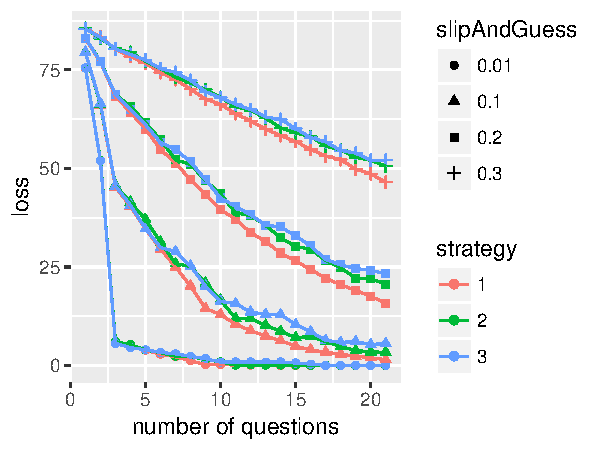
\includegraphics[width=5cm, height=4cm]{Figures/LossStrategyComparisonThreeSkills.pdf}
			\caption{Three Strategy Comparison on 3-skill case}
			\label{fig:Str-1}
		\end{minipage}
		\hfill
	    \begin{minipage}[b]{0.45\linewidth}
	    	\centering
			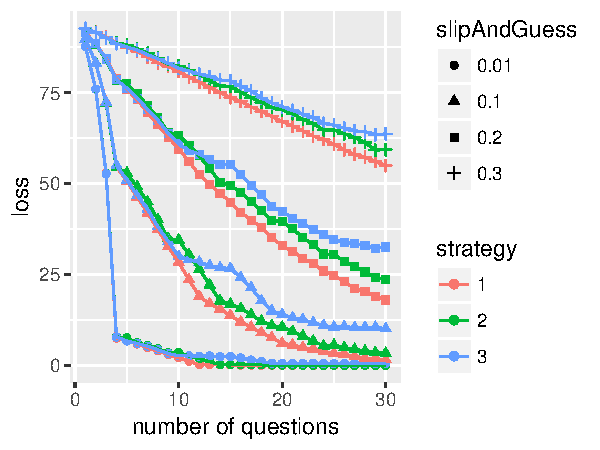
\includegraphics[width=5cm, height=4cm]{Figures/LossStrategyComparisonFourSkills.pdf}
			\caption{Three Strategy Comparison on 4-skill case}
			\label{fig:Str-2}
	    \end{minipage}
	\end{figure}
\end{frame}

\subsection{Experiment 2}
\begin{frame}{Experiment 2}
Find best configuration
\begin{itemize}
\item{A brute force approach}
\item{Given number of skills 3, we have number of q-vectors 7, then for a specific number of questions 4, we have ${{4+7-1}\choose {7-1}}=210$ possible configurations.}
\end{itemize}
\end{frame}

\begin{frame}{Result}
	\begin{figure}
		\begin{minipage}[b]{0.45\linewidth}
			\centering
			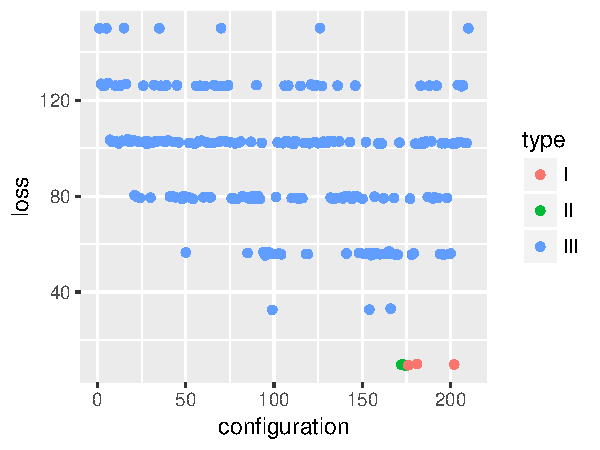
\includegraphics[width=4cm, height=3cm]{Figures/LossBestConfig_theta001_J4.pdf}
			\caption{3-skill case, slip=guess=0.01, J=4}
			\label{fig:Config-1}
		\end{minipage}
		\hfill
	    \begin{minipage}[b]{0.45\linewidth}
	    	\centering
			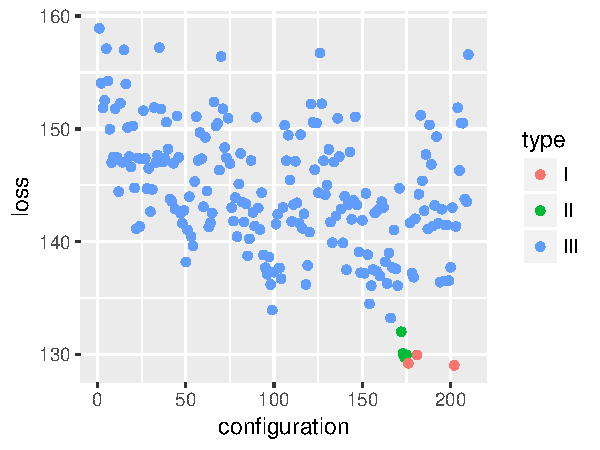
\includegraphics[width=4cm, height=3cm]{Figures/LossBestConfig_theta02_J4.pdf}
			\caption{3-skill case, slip=guess=0.2, J=4}
			\label{fig:Config-2}
	    \end{minipage}
	\end{figure}
\begin{itemize}
\item type I: Complete and confined, meaning it is only consisted of vectors $\{e_{i}:i=1,...,K\}$.
\item type II: Complete but not confined, meaning it not only contains all vectors $\{e_{i}:i=1,...,K\}$, but also contains at least one other q-vector.
\item type III: Incomplete Q-matrix.
\end{itemize}
\end{frame}

\begin{frame}{Result}
	\begin{figure}
		\begin{minipage}[b]{0.45\linewidth}
			\centering
			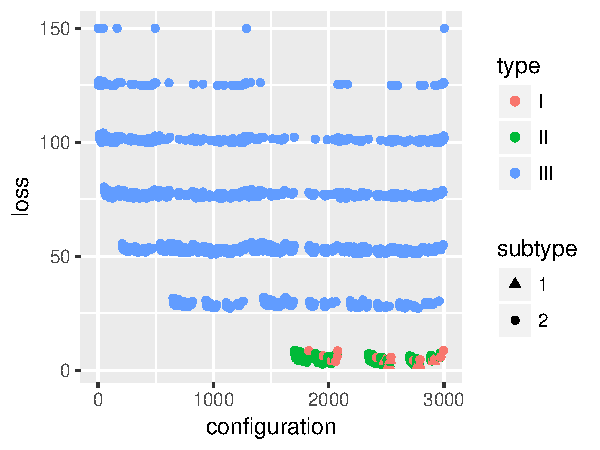
\includegraphics[width=4cm, height=3cm]{Figures/LossBestConfig_theta001_J8.pdf}
			\caption{3-skill case, slip=guess=0.01, J=8}
			\label{fig:Config-3}
		\end{minipage}
		\hfill
	    \begin{minipage}[b]{0.45\linewidth}
	    	\centering
			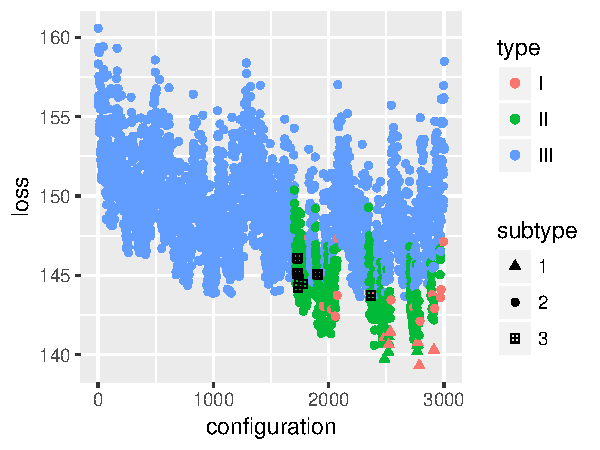
\includegraphics[width=4cm, height=3cm]{Figures/LossBestConfig_theta03_J8.pdf}
			\caption{3-skill case, slip=guess=0.3, J=8}
			\label{fig:Config-4}
	    \end{minipage}
	\end{figure}
\begin{itemize}
\item subtype 1: Q-matrix contains each component of $\{e_{i}:i=1,...,K\}$ at least twice. 
\item subtype 2: Other situations (e.g A complete Q-matrix but all the other vectors are just repeated $e_1$).
\item subtype 3: Q-matrix contains all q-vectors.
\end{itemize}
\end{frame}

\begin{frame}{Result}
	\begin{figure}
		\begin{minipage}[b]{0.45\linewidth}
			\centering
			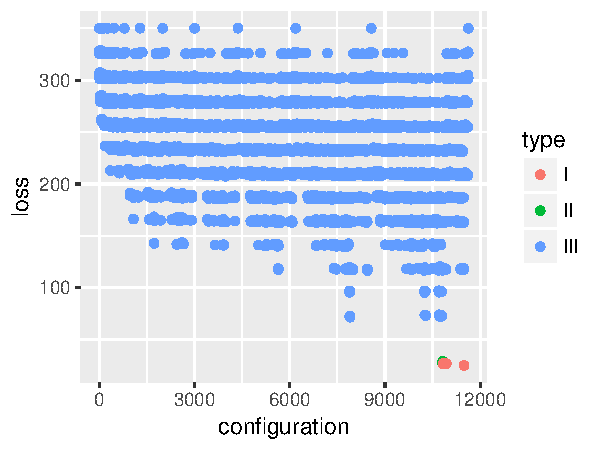
\includegraphics[width=4cm, height=3cm]{Figures/Skill4LossBestConfig_theta001_J5.pdf}
			\caption{4-skill case, slip=guess=0.01, J=5}
			\label{fig:Config-5}
		\end{minipage}
		\hfill
	    \begin{minipage}[b]{0.45\linewidth}
	    	\centering
			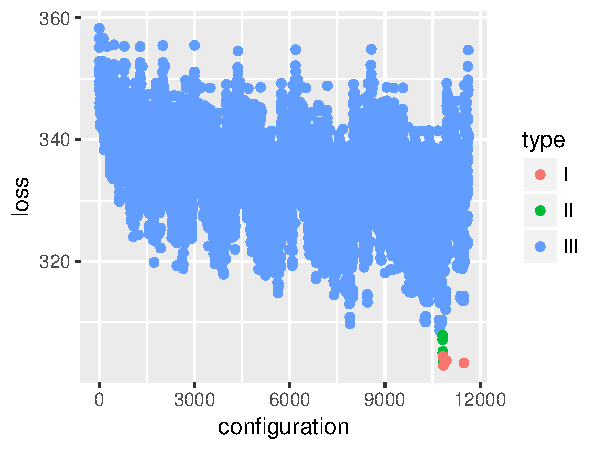
\includegraphics[width=4cm, height=3cm]{Figures/Skill4LossBestConfig_theta02_J5.pdf}
			\caption{4-skill case, slip=guess=0.2, J=5}
			\label{fig:Config-6}
	    \end{minipage}
	\end{figure}
	\begin{itemize}
\item type I: Complete and confined, meaning it is only consisted of vectors $\{e_{i}:i=1,...,K\}$.
\item type II: Complete but not confined, meaning it not only contains all vectors $\{e_{i}:i=1,...,K\}$, but also contains at least one other q-vector.
\item type III: Incomplete Q-matrix.
\end{itemize}
\end{frame}


\section[Conclusion]{Conclusion}
%\begin{frame}{Table of contents}
%\begin{multicols}{2}
%  \tableofcontents[currentsection,hidesubsections]
%\end{multicols}
%\end{frame}

\begin{frame}
	\begin{itemize}
		\item{\textbf{Counter-intuitive:}} A good assessment design should contain items with combination of skills
		\item{\textbf{Synthetic Dataset:}} Impossible to test on real dataset since we do not know the true Q-matrix
		\item{\textbf{Restraints on slip and guess:}} A different identifiability requirement is involved when slip and guess are unknown
	\end{itemize}
\end{frame}

\section[Reference]{Reference}
\begin{frame}{References}
\bibliographystyle{apalike}
\bibliography{biblio.bib}
\end{frame}

\end{document}
